\documentclass[UTF8,a4paper,zihao=-4]{ctexart}

\usepackage[margin=2.4cm]{geometry}
\usepackage{graphicx}
\usepackage{booktabs}
\usepackage{amsmath}
\usepackage{array}
\usepackage{float}
\usepackage{caption}
\usepackage{enumitem}
\usepackage{tikz}
\usetikzlibrary{arrows.meta,positioning,fit,backgrounds}
\usepackage[hidelinks]{hyperref}

\captionsetup{font=small,labelsep=quad}
\setlist{nosep,leftmargin=2em}
\renewcommand{\arraystretch}{1.25}
\hyphenation{Revit BIM HVACIDA}

\title{\heiti 基于 Revit 二次开发的地铁车站机电系统\\BIM 正向设计软件研发与应用}
\author{韩学伟\\[2pt] \small 中铁第六勘察设计院集团有限公司电气化设计院分公司,天津}
\date{}

\begin{document}
\maketitle

\begin{abstract}
\noindent
地铁车站机电系统设计涉及负荷计算、送排风与排烟、水力计算、材料统计和图纸交付等多个环节,现有 BIM 工具在计算口径、模型取值和成果一致性上难以直接满足设计院的生产要求。本文介绍一套在 Revit 2020 上二次开发的机电系统 BIM 正向设计软件:采用 Core(计算内核)/UI(WPF 界面)/Revit(命令与模型交互)三层架构,把院内暖通计算公式逐条移植为可测试的代码,以模型空间为几何数据源,将计算结果、界面表格与 Excel 计算书统一到同一份结果对象。软件包含 7 个功能面板、24 个功能按钮,覆盖大系统负荷与排烟、六类小系统、风/水系统水力计算、材料表与图框出图。以北京站负荷算例和院内六类小系统算例进行逐格校核,总制冷量、总送风量等关键量与原始工作簿一致;并建立 900 余条数值断言与窗口装载自检,保证改动不破坏既有口径。工程应用表明,该软件把重复录入和二次整理的工作量转移到模型与计算书之间的一次性映射上,提高了地铁暖通正向设计的效率与可复核性。
\vspace{0.5em}

\noindent\textbf{关键词:} BIM 正向设计;Revit 二次开发;地铁车站;暖通空调;负荷计算;计算书
\end{abstract}

\section{引言}

城市轨道交通车站的机电设计具有专业多、管线密集、计算依据分散的特点。以暖通专业为例,一个标准站需要完成站厅/站台公共区的大系统负荷与排烟计算、设备管理用房的六类小系统计算、风系统与水系统的水力核算,并输出材料表、图册和计算书。这些工作长期依赖 Excel 表格:几何量从图纸或模型人工抄录,公式散落在多份工作簿中,计算结果再手工整理进计算书,一旦模型调整,整条链路都要重做。

BIM 正向设计要求设计过程以模型为单一数据源。围绕这一目标,已有研究从不同侧面推进:BIM 应用程序接口(API)被用于自动算量与工作区划分\cite{taghaddos2019},IFC 模型被用于规划审查的规则检查\cite{noardo2020},建筑自动化系统数据与运维 BIM 的集成亦有实践\cite{quinn2022}。但在设计院的生产场景中,难点往往不在"能否从模型取数",而在于三件事同时成立:取到的数符合院内计算口径,算完的结果能回到模型与图纸,交付的计算书与界面上看到的是同一份数据。

本文的工作是在 Revit 2020 上开发一套面向地铁车站的机电系统 BIM 正向设计软件(功能区名称 HVACIDA),把上述三件事落成可运行的工程软件,并用可重复的算例回归验证其口径。文章结构如下:第 2 节给出总体设计与模块划分;第 3 节讨论模型取值、公式移植、结果同源与出图四项关键技术;第 4 节给出工程应用;第 5 节报告验证结果与讨论;第 6 节总结。

\section{软件总体设计}

\subsection{分层架构}

软件采用三层架构(图\ref{fig:arch}),层间只通过数据模型与服务接口通信,计算内核不引用 Revit API,因而可以在没有 Revit 的环境下做单元级回归。

\begin{figure}[H]
\centering
\resizebox{0.94\textwidth}{!}{%
\begin{tikzpicture}[
  box/.style={draw,rounded corners=2pt,minimum height=1.05cm,text width=3.5cm,align=center,font=\small},
  layer/.style={draw,dashed,rounded corners=3pt,inner sep=6pt},
  arr/.style={-{Stealth[length=2mm]},thick}
]
\node[box,fill=blue!6] (revit) at (0,0) {HVACIDA.Revit\\App / Ribbon / Command};
\node[box,fill=green!6,right=1.1cm of revit] (ui) {HVACIDA.UI\\WPF 窗口与 ViewModel};
\node[box,fill=orange!8,right=1.1cm of ui] (core) {HVACIDA.Core\\计算、模型、仓库、报告};
\node[box,fill=gray!8,below=1.0cm of revit] (api) {Revit 2020 API\\空间 / 墙 / 图纸};
\node[box,fill=gray!8,below=1.0cm of core] (disk) {local XML\\project / large / small / hydraulic};

\draw[arr] (revit) -- (ui);
\draw[arr] (ui) -- (core);
\draw[arr] (api) -- (revit);
\draw[arr] (core) -- (disk);
\draw[arr,dashed] (revit.south east) -- node[below,font=\scriptsize]{只读拾取} (api.north east);
\end{tikzpicture}}
\caption{软件分层架构}\label{fig:arch}
\end{figure}

Revit 层负责注册功能区、把按钮映射到命令,并完成空间、墙体、图纸等对象的拾取与回写;UI 层是 WPF 窗口与视图模型,只依赖 Core;Core 层实现六类小系统与大系统的全部公式、气象参数库、知识库、Excel 写入器和结果表渲染。三层各自编译为独立程序集,Revit 相关引用以 \texttt{Private=false} 方式引入,不进入输出目录。

\subsection{功能模块}

功能区包含 7 个面板、24 个按钮,与内部模块目录一一对应(表\ref{tab:modules})。模块目录是单一数据源:功能区的按钮顺序、图标、说明窗口和自检清单都从它生成,避免"界面加了按钮、说明没加"的不一致。

\begin{table}[H]
\centering
\caption{功能面板与模块划分}\label{tab:modules}
\small
\begin{tabular}{p{2.2cm}p{6.4cm}p{5.0cm}}
\toprule
面板 & 按钮 & 主要输出 \\
\midrule
项目信息 & 工程信息、气象参数 & 工程档案;大/小系统室外与室内设计参数 \\
大系统 & 公共区参数、负荷计算、排烟计算、计算结果 & 公共区几何与客流;7 个分区负荷;排烟分区与风机选型 \\
小系统 & 全空气一次回风、多联机+新风、排风、送风排风排烟、加压送风、排烟、计算结果 & 六类系统逐房间明细、设备选型与全站汇总 \\
水力计算 & 风系统、水系统、计算结果 & 最不利环路沿程/局部阻力、需求全压与扬程 \\
出图 & 明细表、图框 & 11 类构件材料表;图纸清单与批量导出 \\
AI 问答 & 操作指南、规范知识库、AI 对话、AI 助手 & 口径与条文检索、模型问答(另文讨论) \\
产品支持 & 问题反馈、帮助 & 版本与诊断信息 \\
\bottomrule
\end{tabular}
\end{table}

\subsection{数据组织}

工程数据以 XML 落盘,按用途分为四类:工程与气象(\texttt{project.xml})、大系统负荷与排烟(\texttt{large-system.xml}、\texttt{large-smoke.xml})、小系统工程(\texttt{small-systems.xml})、水力(\texttt{hydraulic.xml})。小系统以"系统类型 + 系统编号"为键存多套,同一类型可有 AHU-A101、AHU-A201 等多套系统,汇总时逐套计算再相加。旧版单系统文件在首次读取时自动迁移,避免升级丢数据。

\section{关键技术}

\subsection{模型对象拾取与几何取值}

Revit 2020 的空间(Space)属于"存在于 API、不在原生对象模型"的类型,直接按类型过滤会抛异常。软件统一以 \texttt{SpatialElement} 收集再筛 \texttt{Space},并在自检中静态扫描源码,禁止该写法回归\cite{revitapi2020}。

拾取分三种粒度:批量识别全模型空间(按名称与标高中的"站厅""站台"分类,同类中优先取名称含"公共区"者);框选指定空间(可多选、回车结束);两点测量(在模型里点起点与终点,取两点距离作为与土壤接触的外墙长度)。拾取到的房间记录来源空间 Id,再次打开窗口时按 Id 重读模型的面积与层高,模型改了,表里的几何量随之更新;空间被删除时保留上次的值并提示。

几何量统一保留 1 位小数,且"界面显示位数 = 参与计算位数":录入框按位数显示并四舍五入写回,避免"表里 4.55、算的时候 4.547"的隐性偏差。

\subsection{计算内核的文档化移植}

计算口径以院内《大系统负荷计算公式》《小系统空调负荷、送排风、排烟计算公式》为准;室外气象数据取自 GB 50736 附录 A\cite{gb50736},车站室内设计参数按 GB 50157 取用\cite{gb50157},排烟量按 GB 51251 的单位面积风量口径复核\cite{gb51251}。移植时遵循三条约束:

\begin{enumerate}
\item \textbf{逐式对应}。每个方法在注释中标注公式在文档中的位置与含义,系数集中定义为常量,便于与文档逐条对照。
\item \textbf{不发明系数}。文档未给出的量不擅自外推;确需补全时(如消除余热通风量在室内温度不高于过渡季温度时的处理)在结果的口径说明中写明,并在界面提示。
\item \textbf{示例只用于理解}。文档中的算例作为回归输入,而不是口径来源;当算例与正文文字不一致时,以正文为准并在结果中说明差异。
\end{enumerate}

以多联机+新风系统为例,房间冷负荷由设备、照明与人员三项构成,消除余热通风量与换气次数通风量取大得到计算通风量,室内状态点由 7 次多项式饱和含湿量与相对湿度确定,新风冷负荷取人员新风量与新风/室内焓差之积并乘管道附加系数。室内机选型按"台数 $\times$ 单台选型冷量"分摊,单台计算冷量在设计人录入台数后按房间冷负荷乘选型系数再除以台数;室外机选型冷量由房间选型冷量合计与新风机组选型冷量相加。上述链条在代码中与示例工作簿的 20 列逐格对应,任一环节改动都会被断言捕获。

\subsection{结果同源与计算书生成}

计算结果先组织为与界面无关的结果表对象(分节、行、单位、小数位),再由三个渲染器分别输出:界面表格、文本计算书、Excel 工作簿。三者读同一份对象,因此不会出现"界面一个数、计算书另一个数"。

Excel 计算书由自写的 XLSX 写入器生成(直接拼装 ZIP 与 XML 部件),不依赖第三方库,与"不引入额外运行时依赖"的约束一致。小系统单套计算书包含计算参数、系统结果、房间明细(带合计行)、设备选型、口径与待补五页;房间明细的列定义与界面参考表共用同一份元数据,列名、顺序与小数位不会分叉。

\subsection{统计与出图}

材料表按"类别 + 族 + 类型 + 单位"归并,单位进入归并键,长度与件数不互相求和;图框模块读取模型中的图纸,列出编号、名称、图框类型、图幅、视图数与是否空图框,支持按 DWG/DXF 逐张导出、PDF 走系统打印机,以及在平面视图中批量标注空间名称与编号。

\section{工程应用}

以某地铁车站为例:站厅公共区 2\,860 m$^2$、站台公共区 1\,980 m$^2$,设 8 个设备管理用房。设计人在公共区参数窗完成空间识别与客流录入后,大系统负荷计算窗按 7 个分区录入围护结构、客流、照明、设备与新风参数,计算结果窗给出计算参数与选型参数两段(图\ref{fig:large})。小系统按房间类型分别建立全空气一次回风与多联机+新风系统,房间表按参考表列出每个房间的逐项计算值(图\ref{fig:vrf}),设计人只需维护面积、人数、设备冷负荷与选型冷量等少量输入。

\begin{figure}[H]
\centering
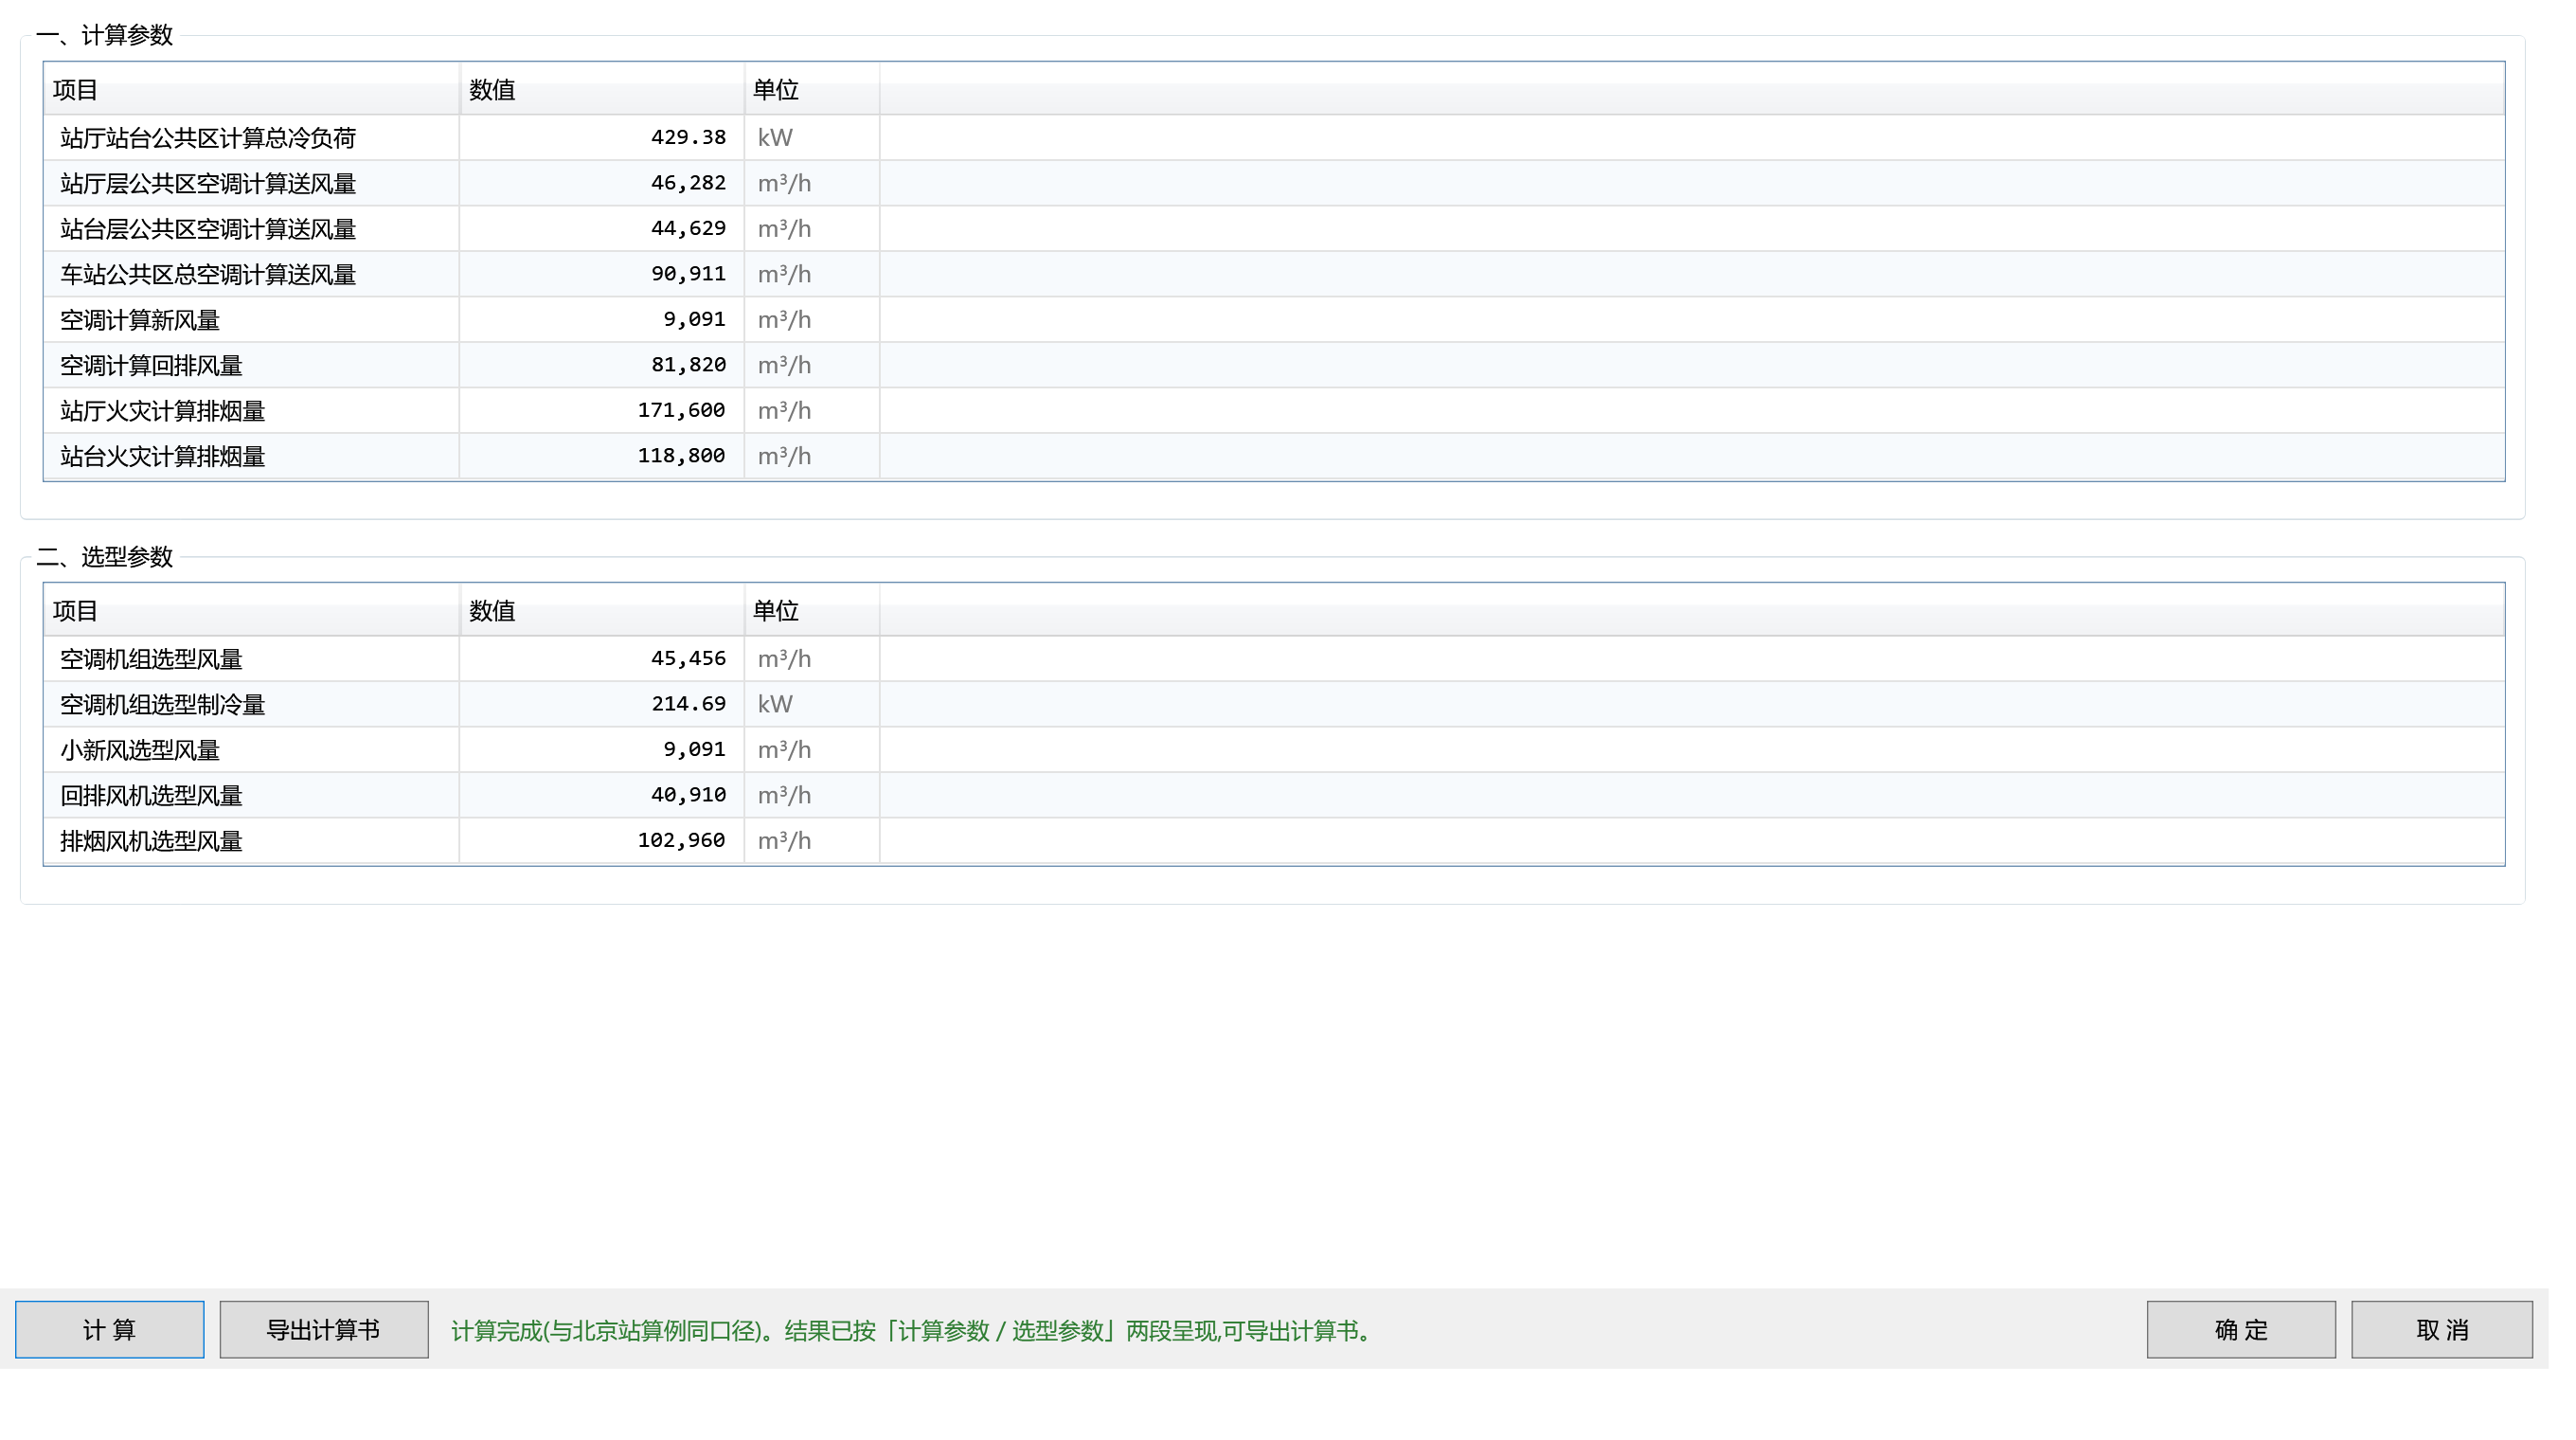
\includegraphics[width=0.95\textwidth]{figures/large-result.png}
\caption{大系统计算结果窗:计算参数与选型参数}\label{fig:large}
\end{figure}

\begin{figure}[H]
\centering
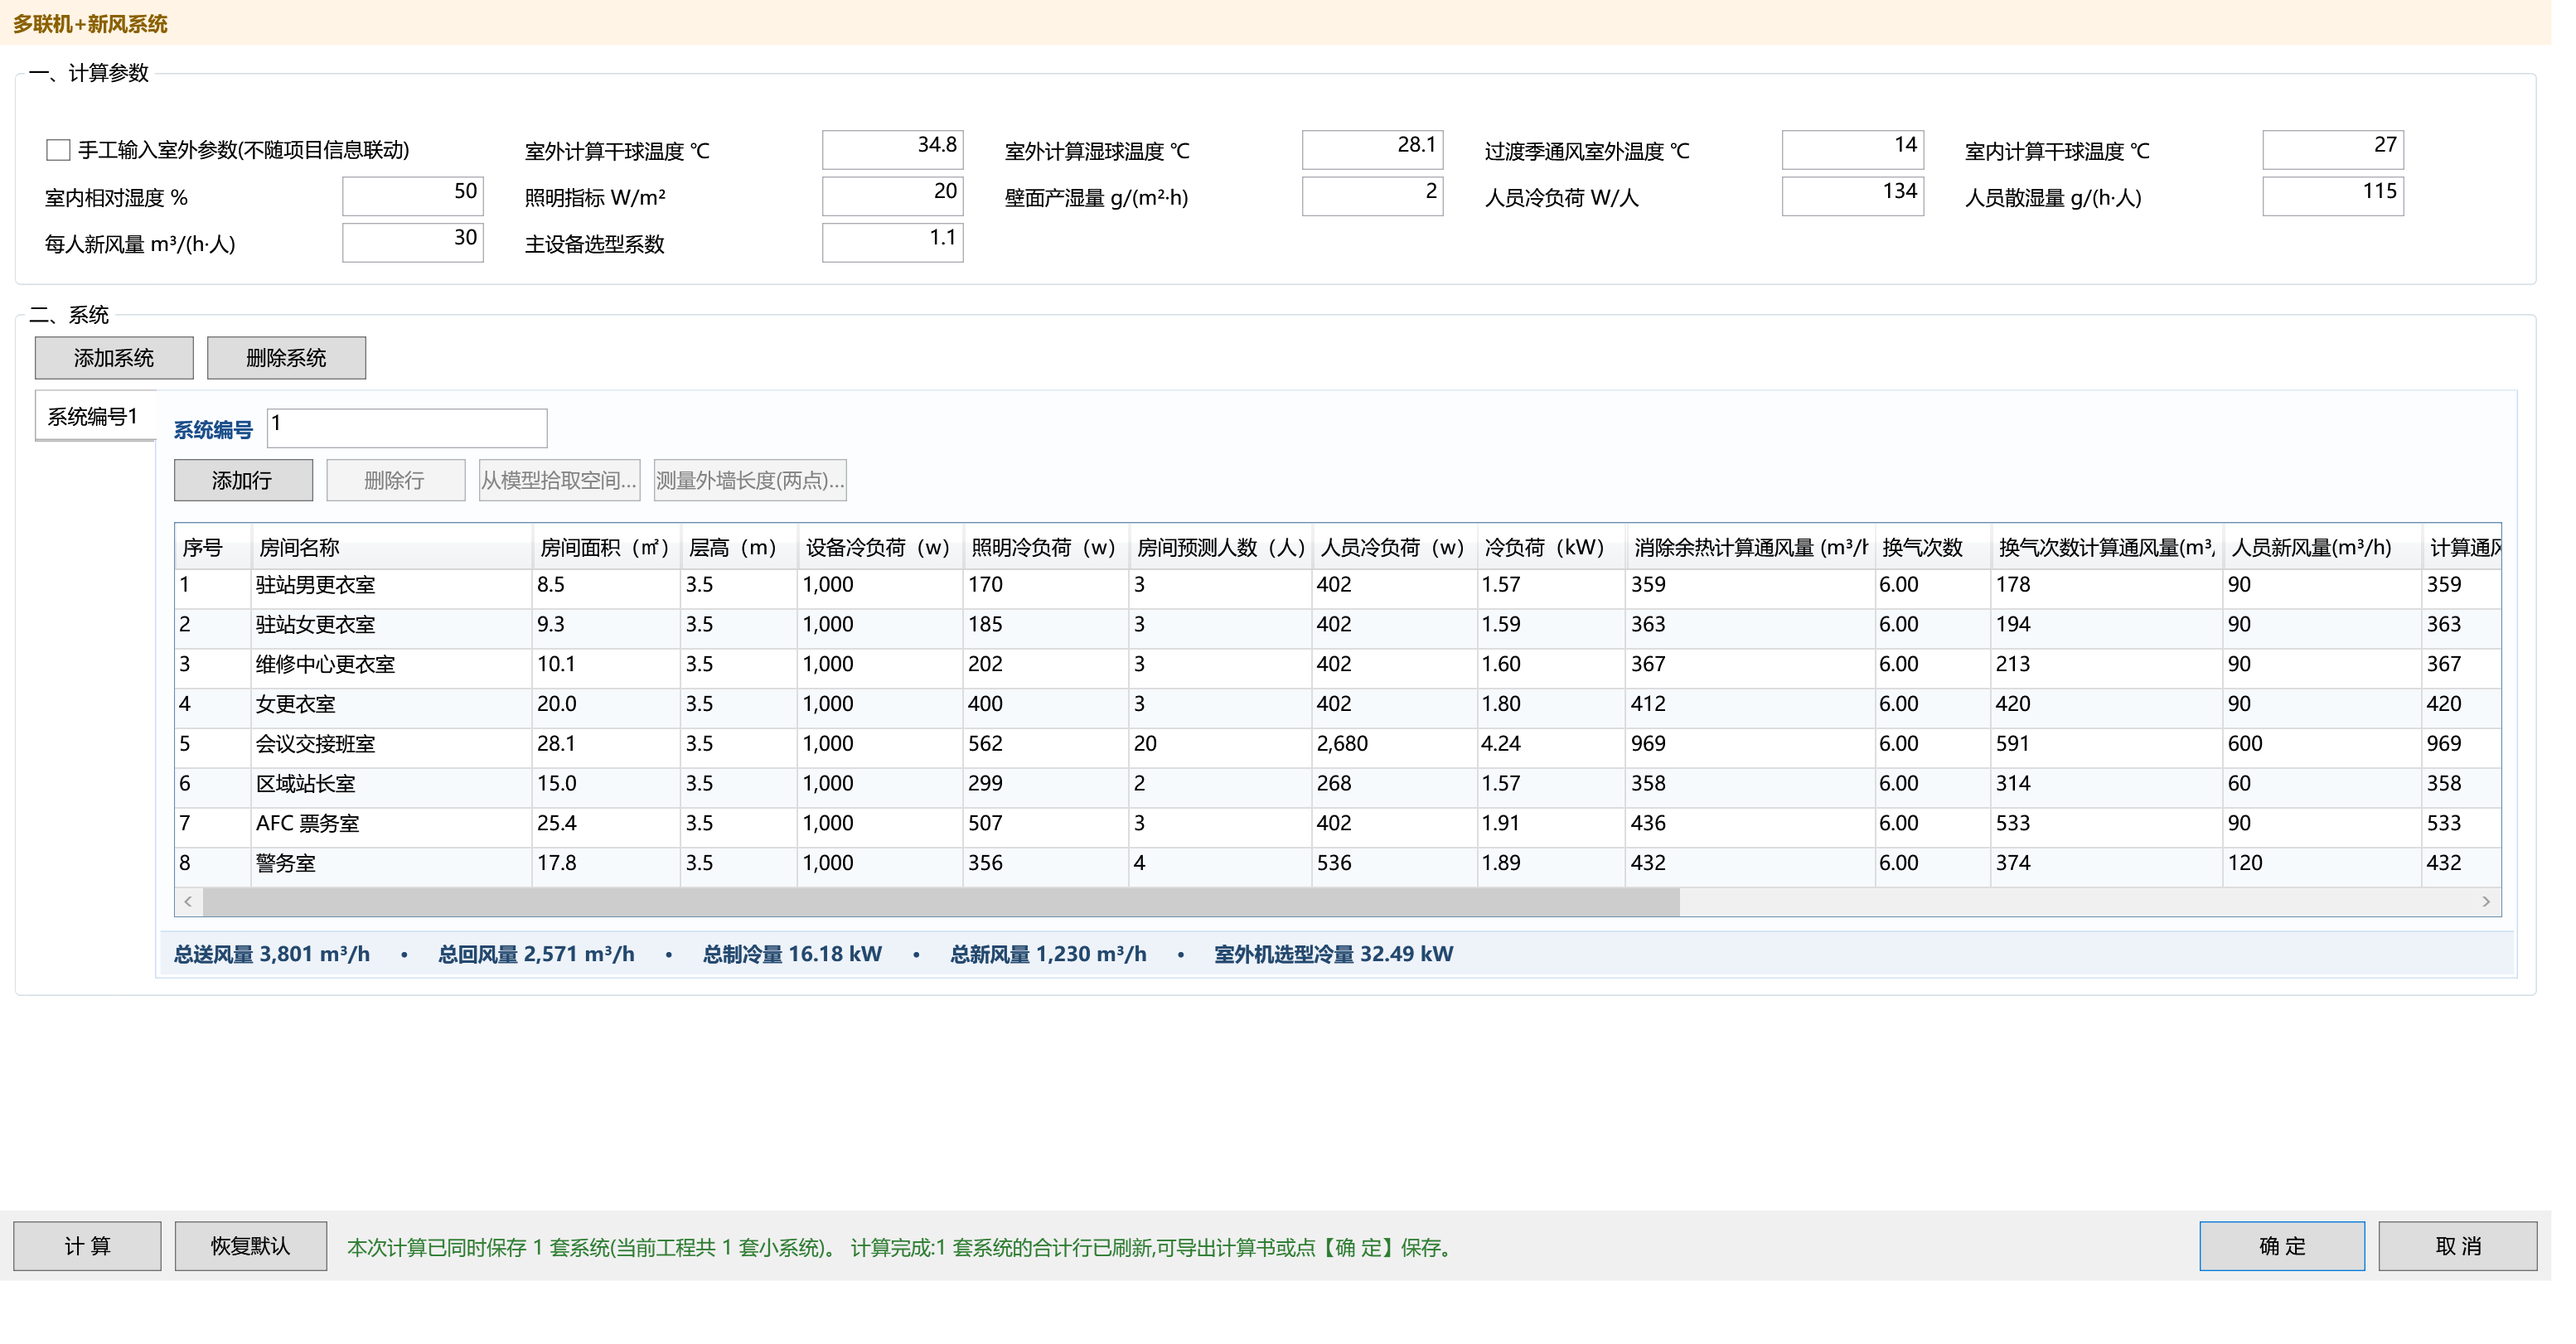
\includegraphics[width=0.95\textwidth]{figures/small-vrf.png}
\caption{多联机+新风系统房间表(20 列,前段可编辑、后段自动计算)}\label{fig:vrf}
\end{figure}

风系统水力计算窗从模型读取管网后,给出最不利环路的沿程与局部阻力、末端与出口动压、计算总阻力与需求全压(图\ref{fig:hyd});水系统同理,需求值换算为扬程。并联环路给出不平衡率与平衡阀 Kv 建议值,阻力特性曲线给出工况点。

\begin{figure}[H]
\centering
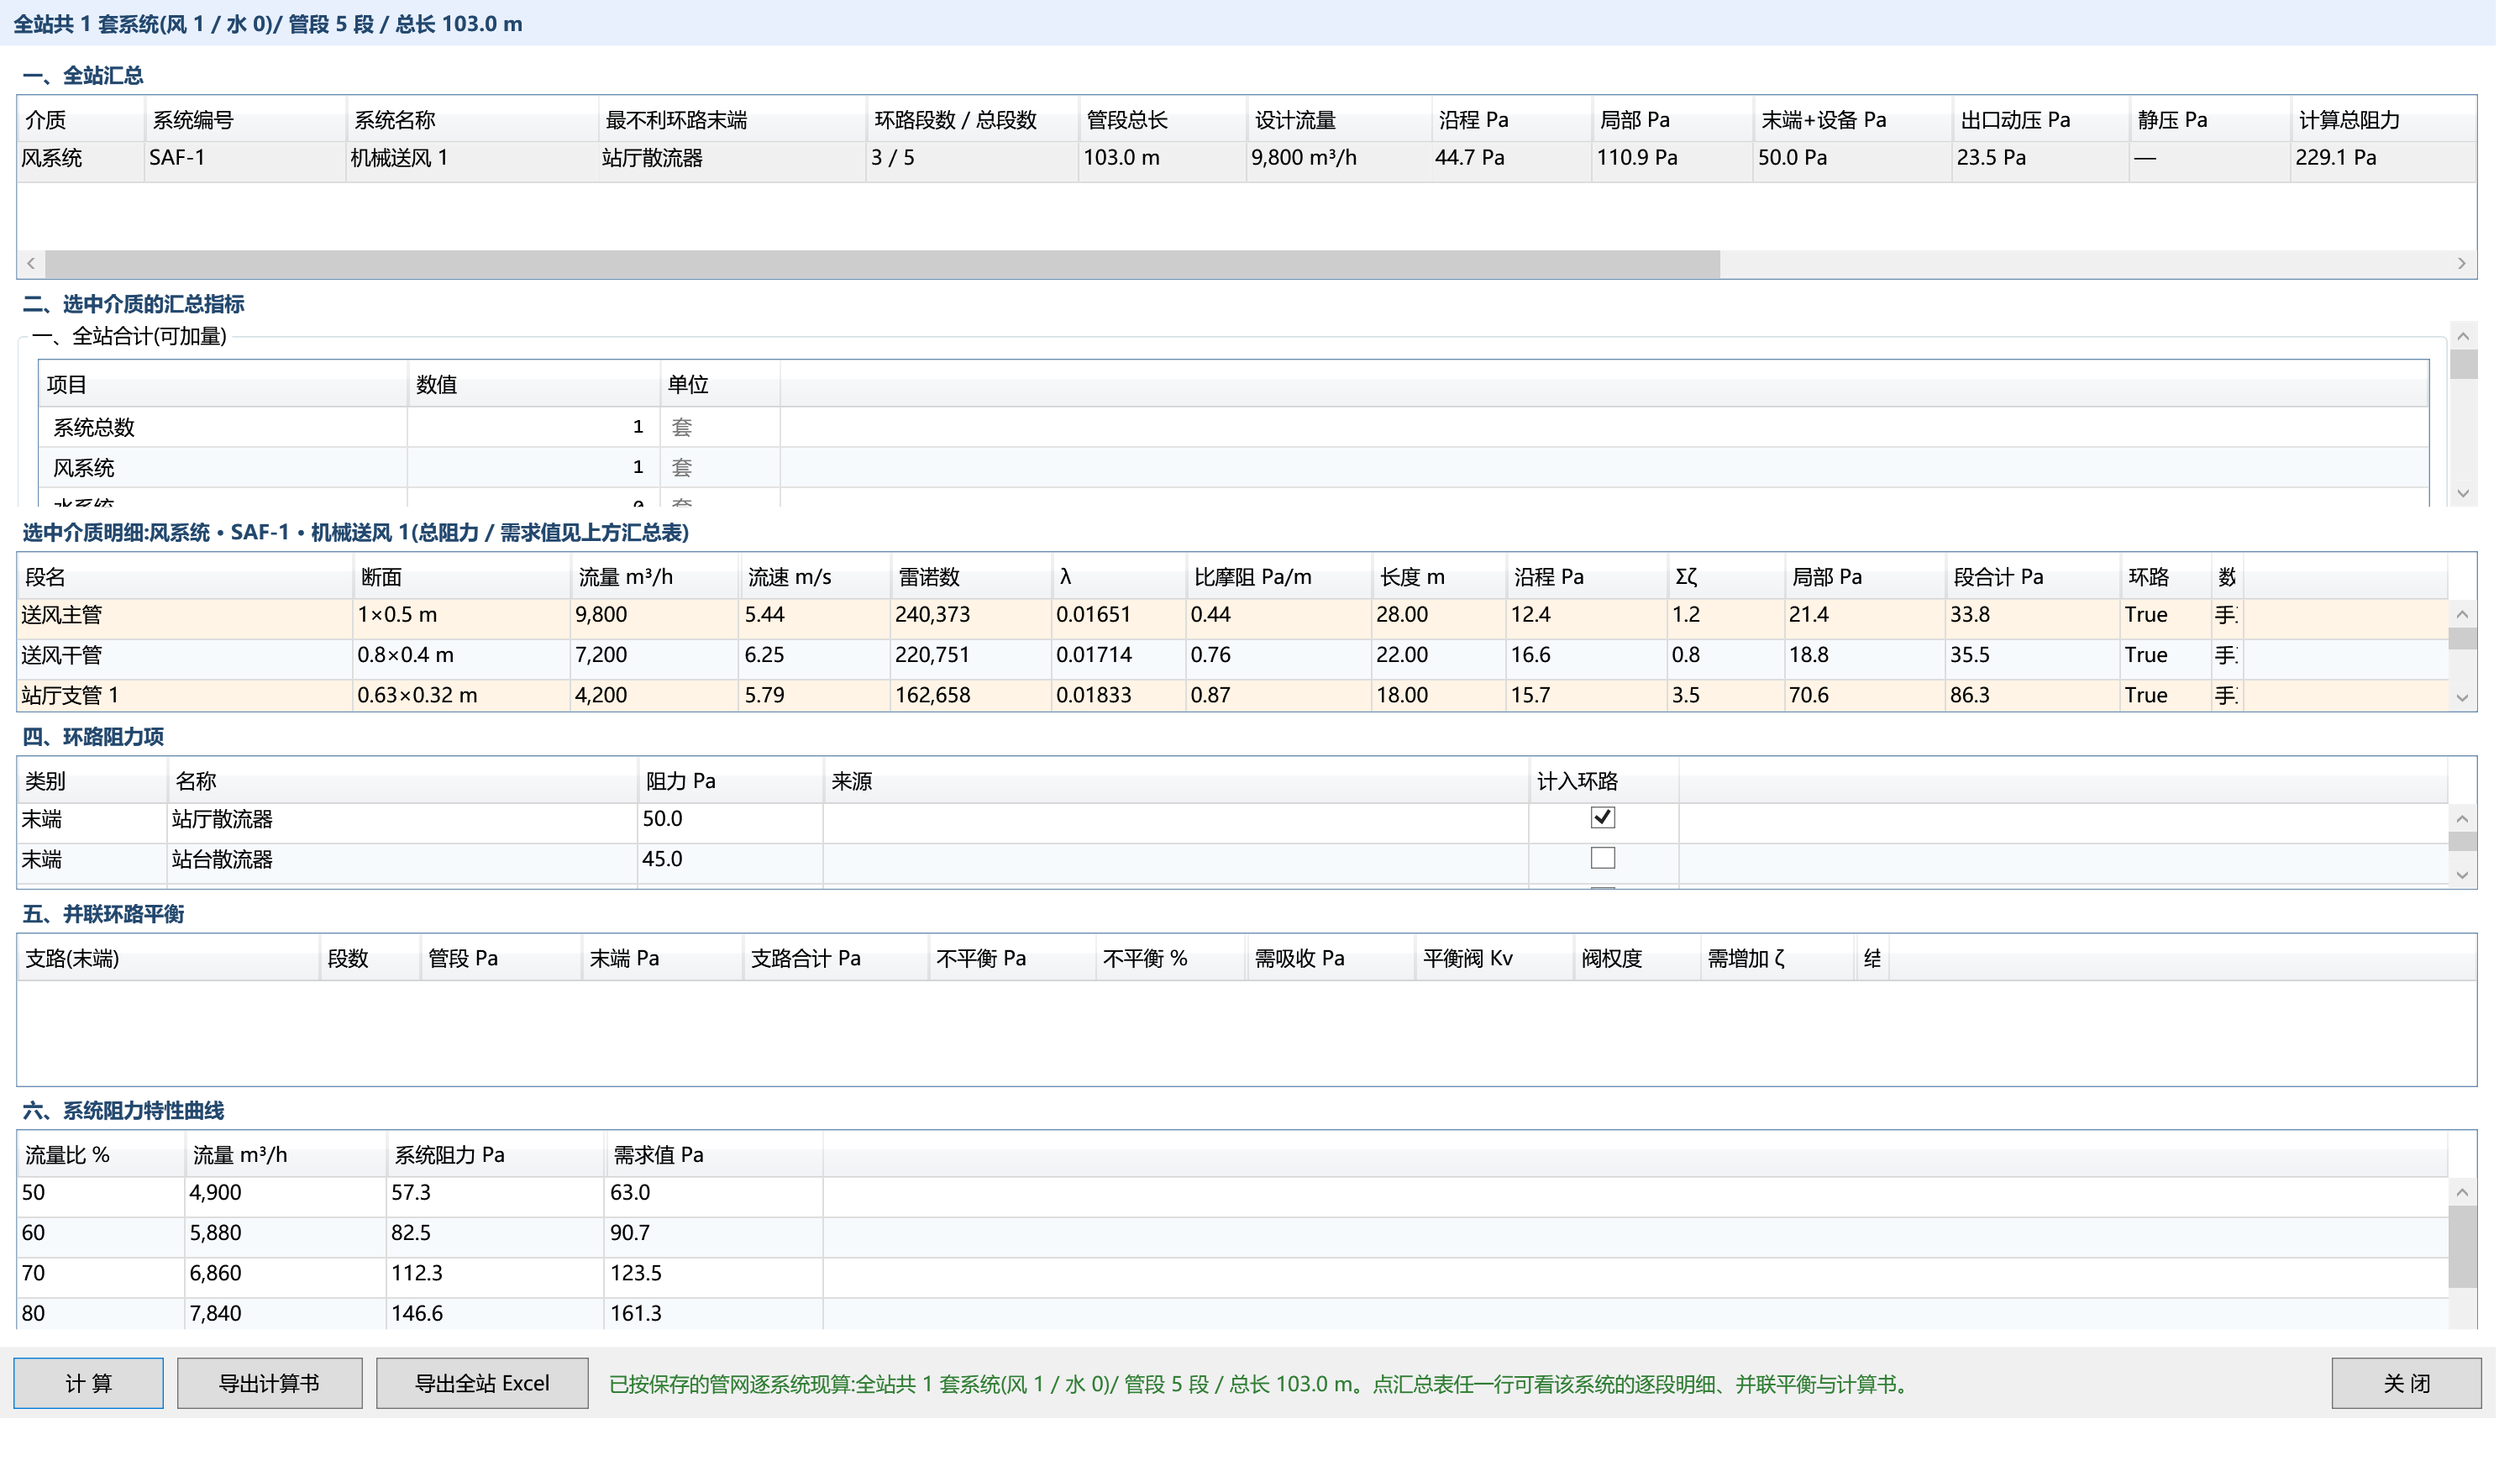
\includegraphics[width=0.95\textwidth]{figures/hydraulic.png}
\caption{水力计算结果:全站汇总、逐段明细与并联平衡}\label{fig:hyd}
\end{figure}

\section{验证与讨论}

\subsection{数值回归}

大系统以北京站算例为回归输入,输入取自院内示例工作簿,对总制冷量、总送风量、各分区冷负荷与湿负荷逐格断言。结果表明总制冷量 381.598 kW、总送风量 87\,768 m$^3$/h 与工作簿一致;剔除气象参数三格(由项目信息联动补入)后,其余各格同样一致。

小系统六类分别以文档示例复算(表\ref{tab:cases})。全空气一次回风的空调器冷量合计为 162.2 kW,文档示例为 157.6 kW,差约 3\%:原因是示例中部分房间的冷量按消除余热通风量取值,而正文规定按计算通风量取值,软件按正文实现并在口径说明中记录该差异。多联机+新风的示例复算给出房间冷负荷合计 15.7336 kW、计算通风量 3\,924.56 m$^3$/h、新风冷负荷 7.0167 kW、室外机选型冷量 27.3184 kW,与示例工作簿逐格一致。

\begin{table}[H]
\centering
\caption{六类小系统的回归算例与关键量}\label{tab:cases}
\small
\begin{tabular}{p{2.6cm}p{5.6cm}p{4.6cm}}
\toprule
系统类型 & 算例规模 & 关键校核量 \\
\midrule
全空气一次回风 & 21 个房间 & 冷负荷 104.42 kW;送风 32\,539 m$^3$/h;空调器冷量 162.2 kW \\
多联机+新风 & 11 个房间(选型另按 7 房间示例) & 冷负荷 21.57 kW;室外机选型 27.3184 kW \\
排风 & 8 个房间 & 计算排风量 5\,386 m$^3$/h \\
排烟 & 2 个防烟分区 & 计算排烟 34\,620 m$^3$/h;补风 20\,772 m$^3$/h \\
送风排风排烟 & 5 个房间 & 排风 20\,307、排烟 31\,020、补风 18\,612 m$^3$/h \\
加压送风 & 楼梯间门参数 & 加压送风量 14\,412.4 m$^3$/h \\
\bottomrule
\end{tabular}
\end{table}

\subsection{软件自检}

数值之外,软件把"能不能打开、绑定是否有效、功能结构是否完整"也做成可执行检查。计算内核的数值与结构自检含 900 余条断言,覆盖六类系统、气象库、材料表、水力、知识库与 AI 助手;窗口自检在无 Revit 的环境下实例化每个窗口,逐条校验 12 个窗口约 450 个数据绑定均可解析,并检查按钮、表格列数与保存行为;功能区自检校验 7 个面板、24 个按钮、24 组 16/32 像素图标齐全且可解码。三套检查在每次提交前运行,任一失败即阻断。

\subsection{讨论}

本文的验证是"口径一致性"验证,回答的是"算出来的数是否等于文档规定",而不是"设计结果是否最优"。后者依赖工程判断,不属于软件职责。软件的局限主要有三点:一是公式以院内文档为准,若文档修订,代码需要同步移植并更新回归基线;二是模型取值依赖空间已放置且已计算体积,未放置空间的面积取不到,需要设计人补录;三是目前仅在 Revit 2020 上验证,高版本的 API 差异(如单位制接口)尚未覆盖。

\section{结论}

本文实现的机电系统 BIM 正向设计软件以三层架构把计算内核与 Revit 解耦,用文档化移植保证计算口径可追溯,用同源渲染保证界面、计算书与 Excel 一致,用可执行的数值与结构自检保证改动可控。北京站负荷算例与六类小系统算例的逐格校核表明,软件的关键计算结果与院内工作簿一致;工程应用表明,设计人可以把精力从"抄数与整理"转向"判断与选型"。后续工作将围绕高版本 Revit 适配、模型回写(把选型结果写回设备参数)以及计算书模板的可配置化展开。


\begin{thebibliography}{9}
\bibitem{taghaddos2019} Taghaddos H, Mashayekhi A, Sherafat B. Automation of construction quantity take-off: using building information modeling (BIM)[J]. arXiv preprint arXiv:1906.02400, 2019.
\bibitem{noardo2020} Noardo F, Wu T, Arroyo Ohori K, et al. IFC models for (semi)automating common planning checks for building permits[J]. arXiv preprint arXiv:2011.03117, 2020.
\bibitem{quinn2022} Quinn C, Zargar Shabestari A, Litoiu M, et al. Building automation system data integration with BIM: data structure and supporting case study[J]. arXiv preprint arXiv:2205.05518, 2022.
\bibitem{revitapi2020} Autodesk. Revit 2020 API developer guide[EB/OL]. https://www.autodesk.com/developer-network/platform-technologies/revit, 2019.
\bibitem{gb50736} 中华人民共和国住房和城乡建设部. 民用建筑供暖通风与空气调节设计规范: GB 50736---2012[S]. 北京: 中国建筑工业出版社, 2012.
\bibitem{gb50157} 中华人民共和国住房和城乡建设部. 地铁设计规范: GB 50157---2013[S]. 北京: 中国建筑工业出版社, 2013.
\bibitem{gb51251} 中华人民共和国住房和城乡建设部. 建筑防烟排烟系统技术标准: GB 51251---2017[S]. 北京: 中国计划出版社, 2017.
\end{thebibliography}

\end{document}
